\documentclass{article}
\usepackage[utf8]{vietnam}
\usepackage{graphicx}
\usepackage{amsmath}
\usepackage{amssymb}
\usepackage{hyperref}
\usepackage{caption}
\usepackage{subcaption}
\usepackage[a4paper, total={6in, 8in}]{geometry}

\title{Some simple tasks in Computer Vision \\ \Large Report Lab Week 19-20}
\author{Ngọc Thuận - IPSAL LAB}
\date{May 2023}
\begin{document}

\maketitle
\begin{abstract}
    Tất cả những gì ta đi qua cũng để phục vụ cho những tác vụ trong thực tế. Trong bài này chúng ta sẽ tìm hiểu về một số tác vụ cơ bản trong Computer Vision, cụ thể là: Object Detection và Semantic Segmentation, với hai mô hình tiêu biểu cho từng bài toán là Faster R-CNN và U-Net.
\end{abstract}
\tableofcontents
\newpage

\section{Tổng quan}
Cũng không cần phải nói nhiều về sự ảnh hưởng của Computer vision trong thực tế và sự tác động mạnh mẽ của các mô hình học sâu đến những đột phá này! Không khó để bắt gặp các tác vụ của Thị giác máy tính như detect trong các xe tự hành, hay phân đoạn các khối u trong sinh học, \ldots Để đạt được những thành công ấy CNN đã mang đến một cuộc cách mạng, ta sẽ cùng tìm hiểu vị trí của các mô hình CNN trong các tác vụ Computer vision trong các mục dưới đây! 
\begin{figure}[ht!]
    \centering
    \begin{subfigure}[b]{0.45\linewidth}
    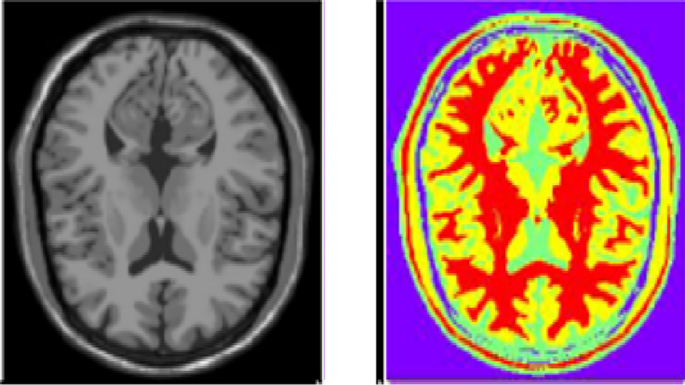
\includegraphics[width = \linewidth]{42979_2021_704_Fig6_HTML.png}
    \caption{Sematic Segmentation}
    \label{fig1a}
    \end{subfigure}
    \begin{subfigure}[b]{0.45\linewidth}
        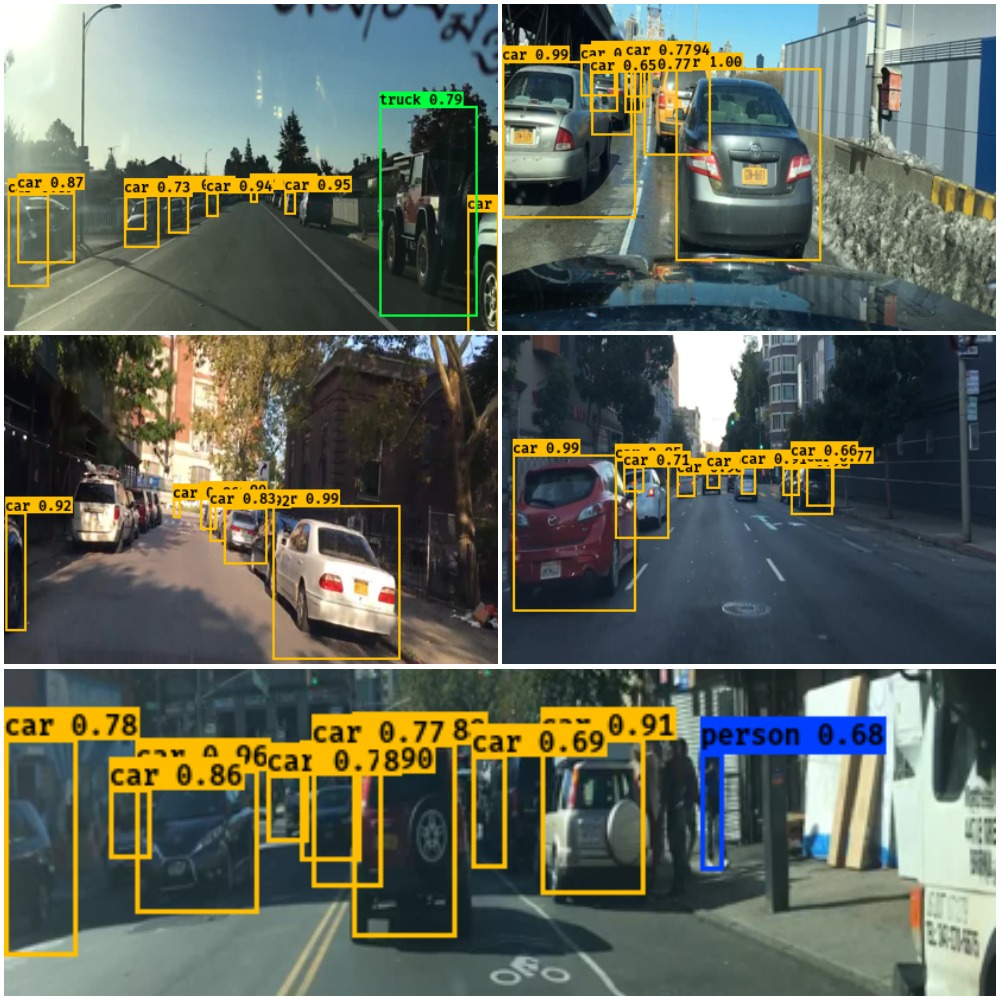
\includegraphics[width = \linewidth]{Test Image Output15a821b.jpg}
        \caption{Object Detection}
        \label{fig1b}
    \end{subfigure}
    \label{fig1}
    \caption{Một số ứng dụng của CV trong thực tế}
\end{figure}

\section{Object Detection}
Đây là một tác vụ cơ bản trong CV với mục đích là xác định ra các vật thể trong một bức ảnh bất kì bằng cách tạo ra các hình chữ nhật gọi là các \textit{bounding boxes} bao quanh vật thể (Ví dụ Hình \ref{fig1b}).

\subsection{Bounding Boxes}
Các bounding boxes có thể được xác định theo 2 cách:
\begin{enumerate}
    \item Tọa độ của góc trên bên trái và tọa độ góc dưới bên phải của hình chữ nhật.
    \item Tọa độ tâm hình chữ nhật và các chiều dài, chiều rộng.
\end{enumerate}
Bounding Boxes chính là các nhãn của các \textit{Object Detection Datasets} bên cạnh nhãn về đề mục (\textit{categories}). Thường sẽ cho theo cách đầu tiên.

\subsection{Anchor Boxes}
Các thuật toán Object Detection thường sẽ lấy mẫu một số lượng lớn các vùng trên ảnh đầu vào, để xác định xem vùng nào có vật thể, từ đó điều chỉnh kích thước các bounding boxes dự đoán. Tùy vào từng mô hình mà có các cách lấy mẫu khác nhau, \textit{anchor boxes} là một trong những phương pháp khá phổ biến. \\\\
Anchor Boxes, dịch ra tiếng việt là các \textit{khung neo}, có đặc điểm là có tâm nằm trên mỗi pixel của ảnh cho trước, chiều dài và chiều rộng tùy chọn.\\\\
Giả sử ảnh đầu vào của ta có chiều dài và chiều rộng là $h$ và $w$. Khi đó chiều dài và chiều rộng của các anchor boxes là $h' = hs/\sqrt{r}$ và $w' = ws\sqrt{r}$. Trong đó $r > 0$ là tỉ lệ khung chứa (VD: 3:4, 1:2, 9:16, \ldots) còn $s \in (0,1]$ là tỉ lệ về độ dài. \\\\Khi lấy mẫu, để tạo ra nhiều anchor boxes với kích thước khác nhau ta sẽ thường cho trước các kích thước $r_1, \ldots, r_m$ và $s_1, \ldots, s_n$. Khi đó các anchor boxes thi được là tổ hợp của các cặp kích thước trên. Tuy nhiên điều này cũng có nhược điểm là sẽ dẫn đến số lượng khung neo quá lớn $h.w.n.m$, trong thực tế ta chỉ cần lấy tổ hợp của $r_1$ và $s_1$. Khi đó số khung neo được tạo ra chỉ còn $h.w.(n+m-1)$ khung neo!
\begin{figure}[ht!]
    \centering
    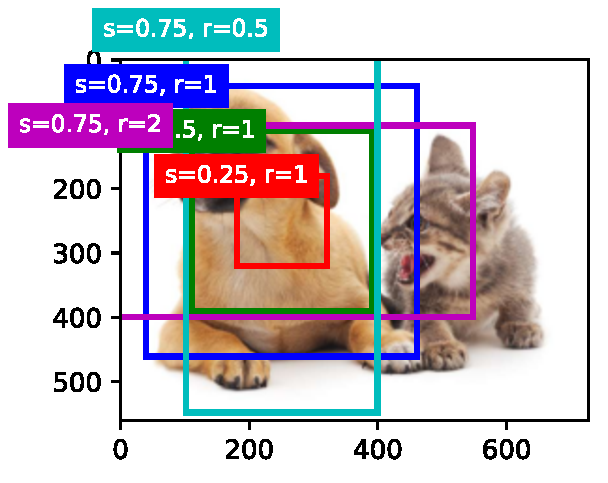
\includegraphics[width = 0.5\linewidth]{output_anchor_f592d1_48_0.pdf}
    \caption{Ví dụ về anchor boxes, Diveintodeeplearning}
    \label{fig2}
\end{figure}

\subsection{Intersection over Union (IoU)}
Xong khâu lấy mẫu, câu hỏi là khi đã có các khung neo, làm như thế nào để xác định một khung neo có vật thể?\\\\
Ta đưa ra khái niệm \textit{Giao trên hợp} (IoU). Khái niệm này bắt nguồn từ \textit{Jaccard index} cho hai tập $A, B$, được định nghĩa như sau:
\begin{equation}
    J(A,B) = \frac{|A\cap B|}{A \cup B}
    \label{eq1}
\end{equation}
Một cách tương tự IoU giữa hai box1 và box2 được định nghĩa như hình \ref{fig3}.
\begin{figure}[ht!]
    \centering
    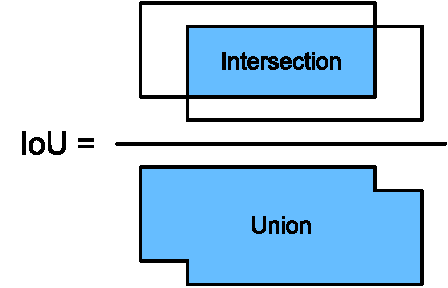
\includegraphics[width = 0.45\linewidth]{iou.pdf}
    \caption{IoU là tỉ lệ giữa vùng giao nhau và toàn bộ vùng của hai bounding boxes}
    \label{fig3}
\end{figure}

\subsection{Nguyên tắc gán nhãn cho các Anchor Boxes}
Tác vụ cuối cùng là gán nhãn cho các anchor boxes.\\\\
Giả sử cho các anchors boxes là $A_1, A_2, \ldots, A_{n_a}$ và các ground-truth bounding boxes là $B_1, B_2, \ldots, B_{n_b}$, hiển nhiên $n_a \geq n_b$. Khi đó ta định nghĩa ma trận $\textbf{X} \in \mathbb{R}^{n_a \times n_b}$ ở đó $x_{ij}$ là IoU của anchor box $A_i$ và grouth-truth bounding box $B_j$. Thuận toán gán nhãn tuân theo các bước sau:
\begin{enumerate}
    \item Tìm phần tử lớn nhất trong ma trận \textbf{X}, ghi lại chỉ số hàng và cột là $i_1, j_1$. Gán nhãn của grouth-truth bouding box $B_{j_1}$ cho anchor box $A_{i_1}$. Sau khi gán, xóa hết các phần tử trên hàng $i_1$ và cột $j_1$.
    \item Tiếp tục tìm phần tử lớn nhất trong ma trận \textbf{X} mới. Làm tương tự như bước 1.
    \item Khi tất cả các cột của ma trận \textbf{X} đã bị xóa tức là ta đã gán xong nhãn cho đủ các ground-truth bouding boxes. Còn lại $n_a - n_b$ anchors boxes, với các anchor boxes $A_i$ còn sót lại tiếp tục tìm $B_j$ có IoU với chúng là lớn nhất, và gán nhãn cho chúng nếu IoU lớn hơn ngưỡng cho trước.
\end{enumerate}
Bây giờ ta đã có thể gán nhãn hạng mục và độ dời cho các khung neo. Giả sử khung neo $A$ mang nhãn của $B$. Khi đó độ dời của $A$ sẽ được gán lại dựa trên sự tương quan giữa $A$ và $B$. Do vị trí và kích thước của các khung trong tập dữ liệu thường khá đa dạng, các vị trí và kích thước tương đối này thường yêu cầu một số phép biến đổi đặc biệt sao cho phân phối của các giá trị độ dời trở nên đều và dễ khớp hơn. Một kĩ thuật phổ biến là gán nhãn của dời của A như sau:
\begin{equation}
    \left(\frac{\frac{x_b-x_a}{w_a} - \mu_x}{\sigma_x}, \frac{\frac{y_b-y_a}{w_a} - \mu_y}{\sigma_y}, \frac{\log{\frac{w_b}{w_a}} - \mu_w}{\sigma_w}, \frac{\log{\frac{h_b}{h_a}} - \mu_h}{\sigma_h} \right)
    \label{eq2}
\end{equation}
Trong đó đầu vào của A, B là các kích thước theo tâm $(x,y,w,h)$ của chúng. Mặc định $\mu_x = \mu_y = \mu_w = \mu_h = 0$, $\sigma_x = \sigma_y = 0.1$ và $\sigma_w = \sigma_h = 0.2$. Nếu một khung neo không được gán nhãn thì khung neo này sẽ được hiểu là nền, sẽ mang nhãn âm. \\\\
Khi lập trình, các khung neo là nền sẽ được gán là nhãn 0, còn các nhãn còn lại sẽ được tăng lên 1.

\subsection{Dự đoán khung chứa với Non-Maximum Suppression}
Khái niệm này ta đã gặp trong thuật toán Canny Detection khi để diễn tả 1 cạnh, nhưng lại có rất nhiều nét. Trường hợp ở đây cũng tương tự, khi có thể sẽ có nhiều khung chứa dự đoán cùng một đối tượng và hiển nhiên sẽ phải chọn ra khung chứa tốt nhất!\\\\
Đây là cách hoạt động của non-maximum suppression. Trong một bức ảnh, tất cả khung dự đoán (hạng mục khác 0) được sắp xếp giảm dần theo $p$ (độ tin cậy - confidence/score, giá trị lớn nhất xác suất cho từng hạng mục của khung chứa dự đoán) vào thành một list $L$. Sau đó ta sẽ làm việc với $L$ theo các bước sau:
\begin{enumerate}
    \item Chọn ra khung chứa $B_1$ có độ tin cậy cao nhất trong $L$ và loại bỏ tất cả những khung chứa có IoU với $B_1$ vượt ngưỡng cho trước ra khỏi $L$. Tức là, $L$ sẽ giữ những khung chứa dự đoán với độ tin cậy cao nhất nhưng loại bỏ những khung chứa quá giống với nó. Đây là ý nghĩa của tên thuật toán non-maximum bị suppressed.
    \item Chọn khung chứa $B_2$ với độ tin cậy cao thứ hai trong $L$, lặp lại bước 1.
    \item Lặp lại cho đến khi tất cả các khung chứa dự đoán trong L đã được duyệt qua. Đến đây thì hai khung chứa dự đoán bất kì IoU đều nhỏ hơn ngưỡng và không cái nào quá giống cái nào.
\end{enumerate}
Sau cùng ta phải trả lại độ dời của các nhãn dự đoán bằng cách giải ngược công thức độ dời \ref{eq2} ở trên.
\begin{figure}[ht!]
    \centering
    \begin{subfigure}[b]{0.45\linewidth}
    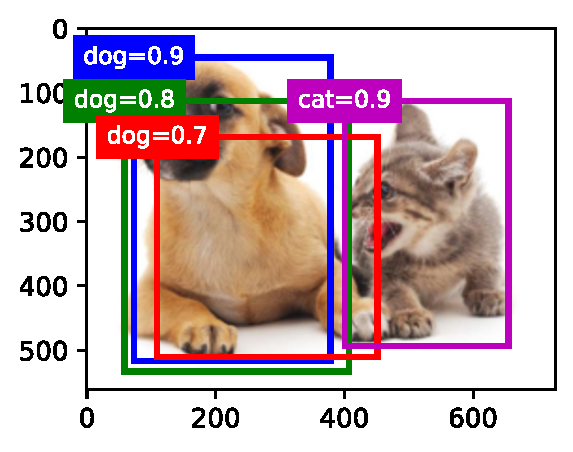
\includegraphics[width = \linewidth]{output_anchor_f592d1_174_1.pdf}
    \caption{Before NMS}
    \label{fig4a}
    \end{subfigure}
    \begin{subfigure}[b]{0.45\linewidth}
        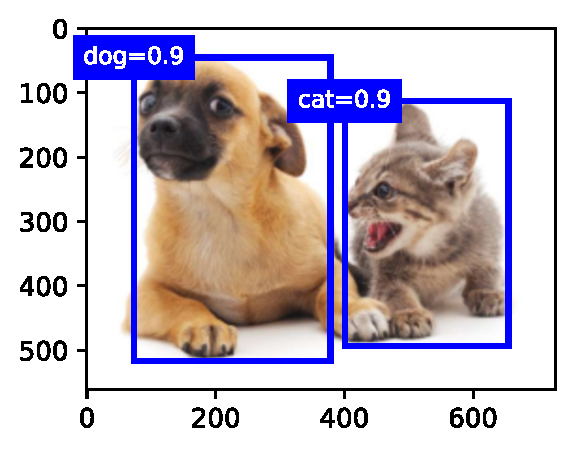
\includegraphics[width = \linewidth]{output_anchor_f592d1_192_1.pdf}
        \caption{After NMS}
        \label{fig4b}
    \end{subfigure}
    \label{fig4}
    \caption{NMS}
\end{figure}

\subsection{Đa kích thước anchor boxes}
Vấn đề của cách tạo anchor boxes bên trên là nó vẫn có thể quá nhiều anchor boxes. Ta có một cách khác để giảm kích số lượng anchor boxes của một bức ảnh vẫn đảm bảo đa kích thước dựa trên feature maps của nó! Thay vì tâm của mỗi anchor boxes là các pixel trên ảnh gốc thì giờ là các pixel trên feature maps. Điều này giúp tạo ra được các anchor boxes với các kích thước khác nhau phân bố đồng đều trên ảnh gốc! Đây là ý tưởng chính của các thuật toán SSD (tham khảo: \href{https://d2l.ai/chapter_computer-vision/ssd.html}{Single Shot Multibox Detection}).

\begin{figure}[ht!]
    \centering
    \begin{subfigure}[b]{0.45\linewidth}
    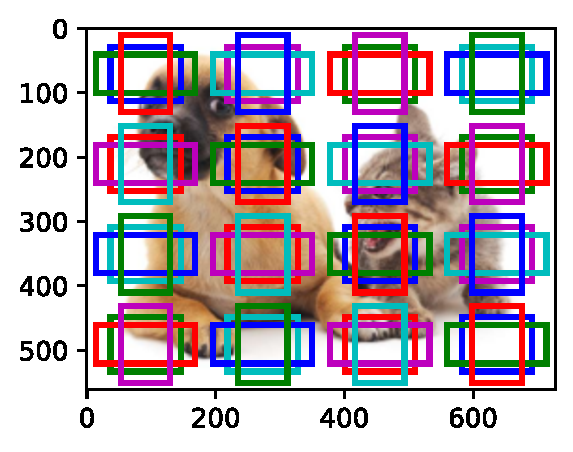
\includegraphics[width = \linewidth]{output_multiscale-object-detection_ad7147_21_0.pdf}
    \caption{4x4}
    \label{fig5a}
    \end{subfigure}
    \begin{subfigure}[b]{0.45\linewidth}
        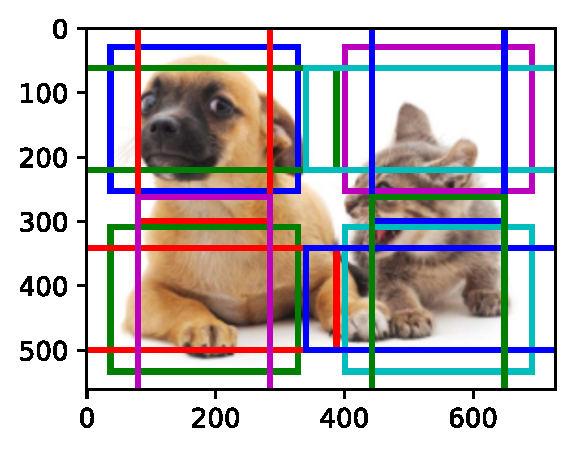
\includegraphics[width = \linewidth]{output_multiscale-object-detection_ad7147_30_0.pdf}
        \caption{2x2}
        \label{fig5b}
    \end{subfigure}
        \begin{subfigure}[b]{0.45\linewidth}
        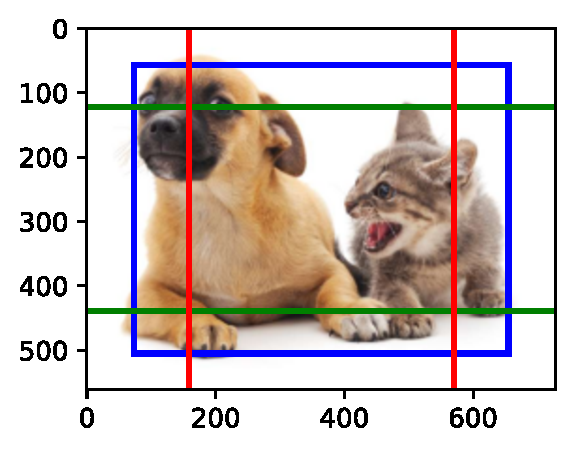
\includegraphics[width = \linewidth]{output_multiscale-object-detection_ad7147_39_0.pdf}
        \caption{1x1}
        \label{fig5c}
    \end{subfigure}
    \label{fig5}
    \caption{Multiscale anchor boxes}
\end{figure}
\subsection{Faster R-CNN}
Đây là một thuật toán thuộc họ \textit{R-CNNs} (region-based CNNs). Đặc điểm của nó là áp dụng các mô hình học sâu lên những vùng đề xuất. Có thể tóm tắt đôi điểm về một số mô hình thuộc series này: 
\begin{enumerate}
    \item R-CNNs, sử dụng thuật toán \textit{selective search} để tạo ra các vùng đề xuất, sau đó coi mỗi vùng đề xuất làm đầu vào của một mô hình học sâu đã được pretrained. Sử dụng SVM để phân loại và linear regression để dự đoán độ dời của khung chứa.
    \item Fast R-CNN, cải thiện hơn khi chỉ còn một mô hình học sâu, song vẫn sử dụng thuật toán \textit{selective search} để tạo ra các vùng đề xuất, sau đó cho đi qua tầng gộp \textit{RoI}, các đặc trưng đầu ra được chia làm 2 đầu ra, một dùng cho tác vụ phân loại hạng mục và một dùng cho tác vụ regression dự đoán độ dời khung chứa.
    \item Faster R-CNN, cải thiện nổi bật nhất so với Fast R-CNN là khối \textit{RPN} thay vì \textit{selective search} để tìm các vùng đề xuất. Tạo thành mô hình end-to-end, tốc độ real-time.
    \item Mask R-CNN, yêu cầu ảnh phải có nhãn cả ở cấp độ điểm ảnh, do phục vụ cả tác vụ Segmentation. Điểm khác biệt ở đây là sử dụng \textit{RoI align}, dùng \textit{bilinear iterpolation} để giữ lại thông tin trong ánh xạ đặc trưng, điều này là vô cùng phù hợp với các dự đoán cấp độ điểm ảnh. Ngoài ra thì có thêm khối \textit{FCN} cho tác vụ phân đoạn ngữ nghĩa.
\end{enumerate}
Tóm tắt là vậy, tuy nhiên ta sẽ chỉ tìm hiểu qua về mô hình số 3. Dưới đây là mô hình tổng quan của Faster R-CNN.
\begin{figure}[ht!]
    \centering
    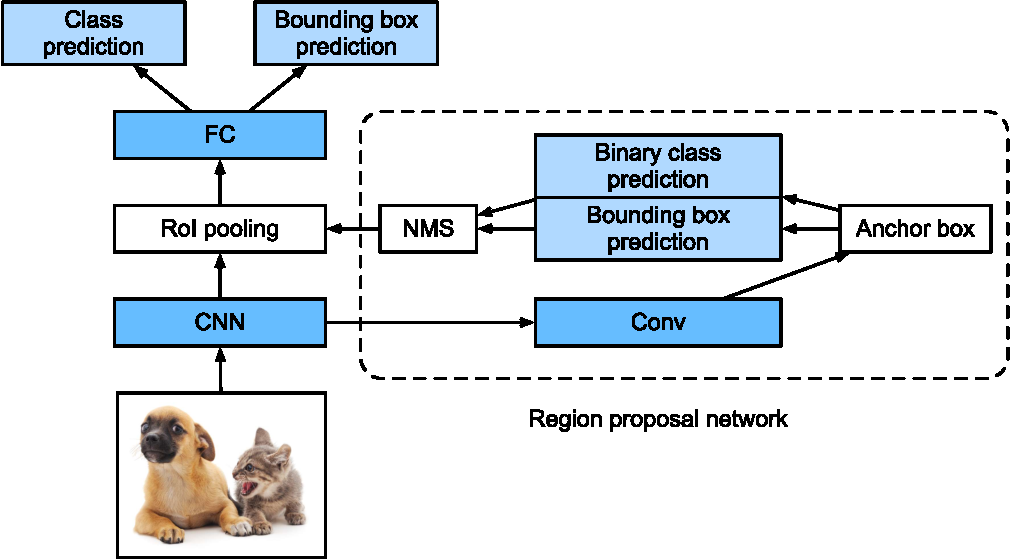
\includegraphics[width = 0.8\linewidth]{faster-rcnn.pdf}
    \caption{Faster R-CNN model, diveintodeeplearning}
    \label{fig6}
\end{figure}
\phantom{a}\\
Lưu ý, NMS mặc dù được xếp trong khối RPN, song thực tế ta phải tách chúng ra, để đảm bảo cho mô hình có thể lan truyền ngược được!

\subsubsection{RoI Pooling}
Trước tiên ta cần tìm hiểu qua về tầng gộp RoI. Khác với các tầng gộp trước đó, ta phải xác định kích thước đầu ra gián tiếp thông qua các kernel. Thì ở gộp RoI ta có thể trực tiếp quyết định đầu ra tầng gộp. \\\\
Giả sử đầu ra của tầng gộp RoI có kích thước là $h_2, w_2$. Khi đó với bất kì đầu vào nào có kích thước $h, w$, thì đầu vào sẽ bị chia thành $h_2\times w_2$ cửa sổ nhỏ, kích thước của mỗi cửa sổ con là sấp xỉ $(h/h_2)\times (w/w_2)$ với đầu ra là phần tử lớn nhất của các cửa sổ con.

\subsubsection{Region propasal network}
Đây có lẽ là phần làm nên sự khác biệt của Faster R-CNN, có nhiệm vụ là đưa ra các vùng đề xuất cho Fast R-CNN của mô hình. Đầu vào là các lower-dimensional features của một mô hình đã qua huấn luyện (256d với ZF và 512d với VGG). Tiếp theo là tầng tích chập $3\times3$ padding 1, và $1\times 1$ được tách ra thành 2 tầng kết nối đầy đủ, box-regression và box-classification. \\\\
Anchor boxes được tạo từ output của tầng tích chập với sizes và ratios được định nghĩa trước, giả sử là $k$ anchor boxes trên mỗi pixel. Khi đó đầu ra của box-regression layer là $4k$ còn đầu ra của box-classification là $2k$.
\begin{figure}[ht!]
    \centering
    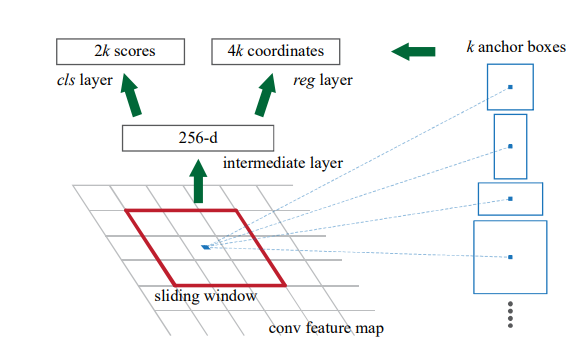
\includegraphics[width = 0.7\linewidth]{rpn1.png}
    \caption{Region Proposal Network (RPN)}
    \label{fig7}
\end{figure}

\subsubsection{Loss Function}
Nhận xét rằng, Faster R-CNN có hai hàm mất mát ứng với hai mô hình cấu tạo nên nó! Đó là RPN và Fast R-CNN, ta có thể dùng cùng một hàm mục tiêu cho cả hai mô hình.\\\\
Việc gán nhãn cho các anchor boxes ta đã giới thiệu ở trên, với quy ước nhãn 0 cho background (anchor âm), nhãn dương cho các khung neo chứa vật thể. Với các định nghĩa có sẵn, ta đi tối thiểu hàm mục tiêu đã được giới thiệu trong Fast R-CNN:
\begin{equation}
    L({p_i}, {t_i}) = \frac{1}{N_{cls}} \sum_{i}L_{cls}(p_i, p^{*}_{i}) + \lambda \frac{1}{N_{reg}}\sum_{i} p^{*}_i L_{reg}(t_i, t^{*}_i)
    \label{eq3}
\end{equation}
Trong đó, $i$ là chỉ số của khung neo trong một mini-batch, $p_i$ là xác suất để anchor $i$ là vật thể, $p^{*}_i$ là nhãn gốc bằng 1 với các anchor dương, bằng 0 với các anchor âm. $t_i$ là độ dời dự đoán của khung chứa, $t^{*}_i$ là nhãn gốc được gắn với các anchor dương.\\\\
Hàm mất mát cho Fast R-CNN, cũng tương tự (\ref{eq3}), tuy nhiên $p_i$ là vector xác suất hạng mục đầu ra của toàn bộ mô hình.\\\\
Ở đây $L_{cls}$ có thể sử dụng \textit{Cross Entropy Loss} hoặc sử dụng \textit{Focal loss}, $L_{reg}$ có thể sử dụng \textit{$l_1$} hoặc \textit{smoth $l_1$}.
\begin{equation}
    Focal\text{ }loss = -\alpha (1-p_j)^\gamma \log{p_j}
    \label{eq4}
\end{equation}

\begin{equation}
    Smoth\text{ }l_1 = \begin{cases}
    (\sigma x)^2/2, & \text{if} |x|<1/\sigma^2\\
    |x|-0.5/\sigma^2, & \text{otherwise}
    \end{cases}
\end{equation}

\subsubsection{Training}
Ta biết rằng hoàn toàn có thể huấn luyện độc lập cả RPN và Fast R-CNN, tuy nhiên điều đó sẽ làm thay đổi tầng tích chập của chúng theo nhiều cách. Do đó chúng ta cần một kĩ thuật cho phép chia sẻ các tầng tích chập giữa 2 mạng, thay vì huấn luyện một cách độc lập. Ở đây có các cách như sau: 
\begin{enumerate}
    \item Alternating training. Theo cách này thì đầu tiên chúng ta sẽ train RPN, sau đó sử dụng các vùng đề xuất của RPN để train Fast R-CNN. Mô hình sẽ được tinh chỉnh bởi Fast R-CNN sau đó được dùng để để tạo RPN, quá trình này được lặp lại. Bài báo gốc sử dụng phương pháp này.
    \item Joint training. Theo cách này, RPN và Fast R-CNN được gộp thành một mạng khi huấn luyện.
\end{enumerate}
Bài báo gốc chia làm 3 phương án nhưng khá phức tạp! Ta cũng có thể kết hợp cả hai cách làm trên. Đầu tiên ta sẽ huấn luyện RPN sau đó huấn luyện kết hợp RPN và Fast R-CNN, hàm mất mát bằng $L_{RPN}+\lambda L_{Fast}$. Đây là cách làm của tôi, code Pytorch có thể tìm thấy ở \href{https://github.com/thuantn210823/Computer-Vision-IPSAL-LAB-}{đây}

\begin{figure}[ht!]
    \centering
    \begin{subfigure}[b]{0.45\linewidth}
    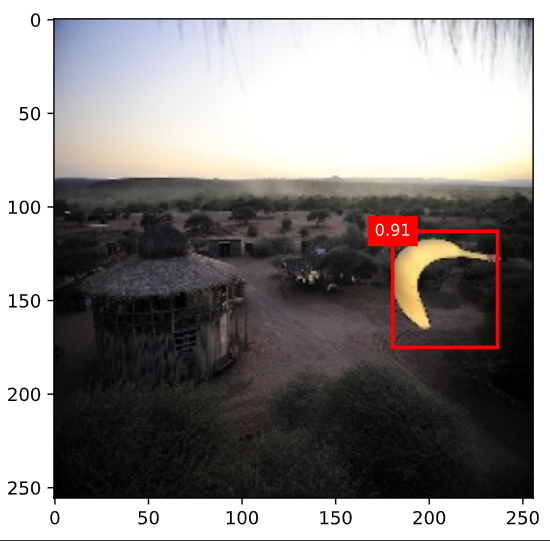
\includegraphics[width = \linewidth]{Screenshot 2023-05-26 213119.png}
    \label{fig8a}
    \end{subfigure}
    \begin{subfigure}[b]{0.45\linewidth}
        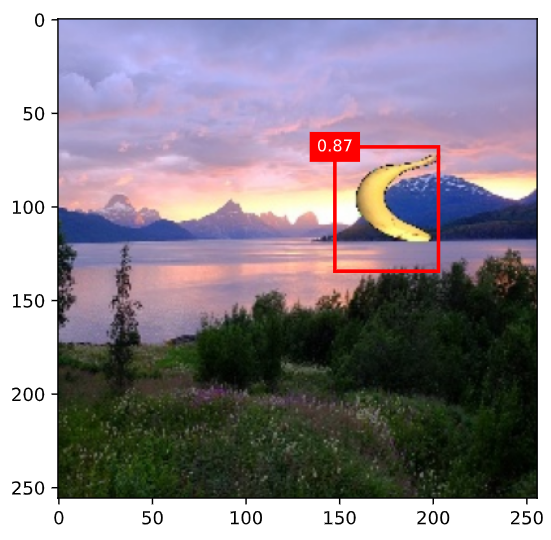
\includegraphics[width = \linewidth]{Screenshot 2023-05-26 213145.png}
        \label{fig8b}
    \end{subfigure}
        \begin{subfigure}[b]{0.45\linewidth}
        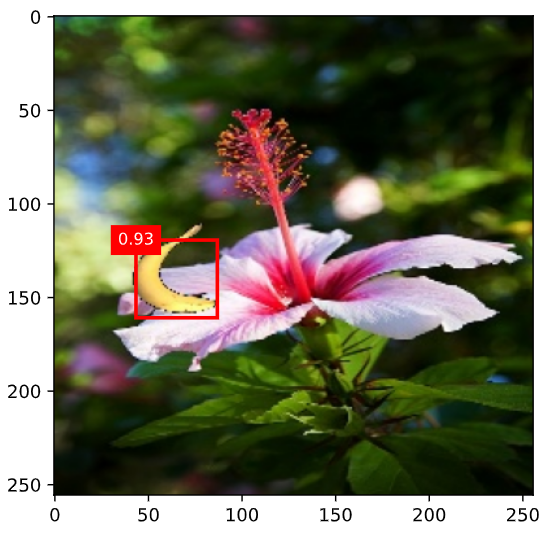
\includegraphics[width = \linewidth]{Screenshot 2023-05-26 213210.png}
        \label{fig8c}
    \end{subfigure}
        \begin{subfigure}[b]{0.45\linewidth}
        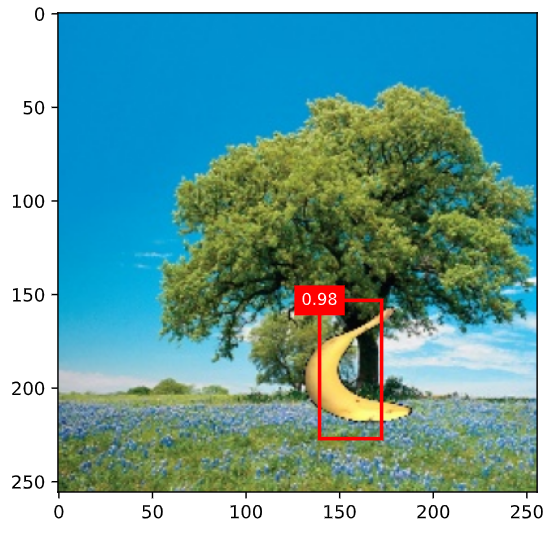
\includegraphics[width = \linewidth]{Screenshot 2023-05-26 213230.png}
        \label{fig8d}
    \end{subfigure}
    \label{fig8}
    \caption{Một số kết quả dự đoán trên Banana Detection Dataset}
\end{figure}
\section{Semantic Segmentation}
Khi nói vể Object Detection ở mục trên ta nói về những khung chứa hình chữ nhật cho việc gán nhẵn và dự đoán vật thể trong bức ảnh. Sang mục này chúng ta sẽ thảo luận về \textit{semantic segmentation}, một tác vụ hướng tới việc chia bức ảnh thành những đoạn khác nhau. Khác với Object Detection, Semantic Segmentation làm việc ở \textit{cấp độ điểm ảnh}: gán nhãn và dự đoán ở cấp độ điểm ảnh.
\\\\
Ở đây có hai tác vụ thị giác máy tính quan trọng khá giống với semantic segmentation là: \textit{image segmentation} và \textit{instace segmentation}. Chúng ta sẽ phân biệt một cách ngắn gọn hai tác vụ này:
\begin{enumerate}
    \item \textit{Image segmentation} chia một bức ảnh thành một vài vùng thành phần. Phương pháp cho loại tác vụ này là dựa trên sự tương quan giữa các pixels trên bức ảnh. Và nó không cần gán nhãn ở cấp độ điểm ảnh trong quá trình huấn luyện, và nó cũng không đảm bảo sẽ phân đoạn như chúng ta mong muốn
    \item {Instace segmentation} còn được gọi là \textit{đồng thời xác định và phân đoạn (simultaneous detection and segmentation)}. Nó học cách nhận biết các vùng cấp điểm ảnh của từng đối tượng trong một hình ảnh. Khác với sematic segmentation, instace segmentation cần phải phân biệt được không chỉ về ngữ nghĩa mà còn phải phân biệt được các vật thể khác nhau. Ví dụ, nếu có hai con chó trong cùng một bức ảnh, instace segmentation cần phải phân biệt được riêng rẽ hai con chó đó!
\end{enumerate}

\subsection{Transposed Convolution}
Khi mới bắt đầu vào các mô hình học sâu ta đã được làm quen với các tầng tích chập, chúng có nhiệm vụ đổi chiều dài, chiều rộng (downsample) lấy kích thước chiều kênh, hoặc giữ chúng không đổi. Tuy nhiên ở các tác vụ phân đoạn với việc phải phân loại ở cấp độ điểm ảnh, ta cần ảnh đầu ra có kích thước giống ảnh đầu vào. Hãy tưởng tượng, đầu ra của ta có kích thước bằng ảnh đầu vào, ở đó mỗi pixel đầu ra là những vector chứa thông tin về hạng mục cho vector đó.\\\\
Để làm được điều này, sau các bước downsample bởi các tầng tích chập ta cần tăng dần kích thước chiều dài, rộng của các ánh xạ đặc trưng (upsample). Trong mục này, ta sẽ tìm hiểu về phép \textit{tích chập chuyển vị}.\\\\
Cách hoạt động cơ bản của phép tích chập chuyển vị có thể được minh họa trong hình \ref{fig9}.
\begin{figure}[ht!]
    \centering
    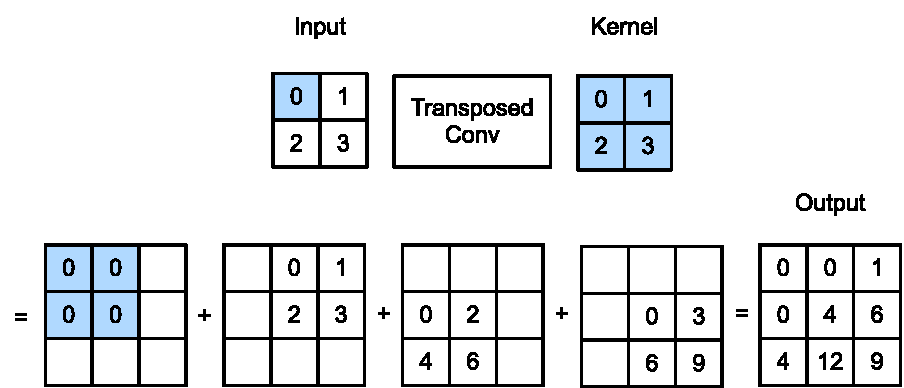
\includegraphics[width = 0.7\linewidth]{trans_conv.pdf}
    \caption{Basic operation}
    \label{fig9}
\end{figure}
\\\\
Từng phần tử ở input được nhân với kernel, các vị trí ở các cửa sổ trung gian được gán tương ứng với vị trí của phần tử input nhân kernel. Đầu ra bằng tổng các cửa sổ trung gian.\\\\
Ở đây cũng có đệm, sải bước và đa kênh vào, đa kênh ra. Tất cả đều ngược lại với phép tích chập thông thường, trừ đa vào đa ra giống! Tức là ở đệm, thay vì padding ở input, chúng ta sẽ remove ở output, sải bước, thay vì thay đổi bước sải ở input ta sẽ thay đổi bước sải ở output!\\\\
Còn về cái tên tích chập chuyển vị (transposed convolution). Bản chất của các tầng tích chập là các tầng kết nối đầy đủ với ma trận trọng số là các ma trận thưa (sparse matrix), trong đó các tầng tích chập thông thường được định nghĩa với phép lan truyền thuận. Khi đó khi lan truyền ngược, ứng với phép lấy gradient theo đầu vào, \textit{ma trận trọng số của ta bị chuyển vị}, và tầng tích chập đầy đủ cho phép lan truyền ngược này lại chính là tầng tích chập chuyển vị!\\\\
Tham khảo thêm ở đây: \href{https://d2l.ai/chapter_computer-vision/transposed-conv.html}{transposed convolution - diveintodeeplearning}.\\\\
\subsection{U-Net}
Bắt nguồn từ một bài báo năm 2015 của Olaf Ronneberger, \textit{et al} cho phân đoạn hình ảnh sinh học. Tuy nhiên là một mô hình tốt U-Net không chỉ dừng lại ở các tác vụ phân đoạn sinh học mà còn trở thành một trong những mô hình phân đoạn ngữ nghĩa phổ biến nhất!
\begin{figure}[ht!]
    \centering
    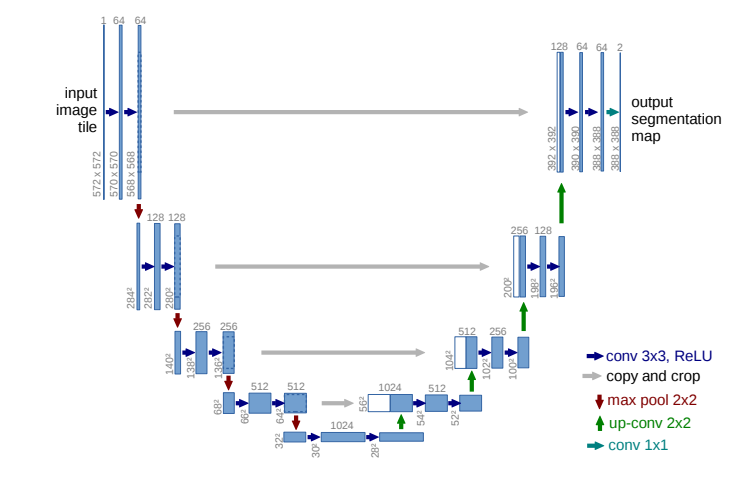
\includegraphics[width = 0.9\linewidth]{unet.png}
    \caption{U-net architecture}
    \label{fig10}
\end{figure}\\\\
Cấu trúc của U-Net được minh họa trong hình \ref{fig10}. Nó chứa hai phần một là \textit{contracting path} (bên trái) và phần còn lại là \textit{expansive path} (bên phải). Contracting path tương tự với các cấu trúc mạng neuron tích chập thông thường. Nó chứa 3 tầng tích chập $3\times 3$ không padding, theo sau là hàm kích hoạt ReLU và tầng gộp cực đại $2 \times 2$. Ở mỗi bước downsampling ta tăng gấp đôi số lượng kênh đầu ra. Mỗi bước ở expansive path chứa một tầng tích chập upsample $2 \times 2$ giảm đi một nửa số lượng kênh của các ánh xạ đặc trưng, sau đó được nối tương ứng với đặc trưng đã được cắt bớt tương ứng bên contractiong path, và hai phép tích chập $3 \times 3$, theo sau là hàm kích hoạt ReLU. Tầng cuối cùng là tầng tích chập $1 \times 1$ để điều chỉnh số kênh đầu ra thành số lượng classes. Tổng tất cả mạng chứa 23 tầng tích chập.\\\\
Lưu ý, theo bài báo gốc thì ảnh đầu vào cần phải được tile (overlap-tile strategy) (padding theo chế độ reflect).\\\\
Tuy nhiên, với mô hình trên mô hình lại trở nên quá phức tạp đối với môi trường nghiên cứu. Có một số biến thể có thể được chấp nhận như, ta sẽ giữ nguyên ảnh đầu vào, thêm padding ở các tầng tích chập, giảm độ sâu và upsample bằng các phương pháp nội suy!
\subsubsection{Loss Function}
Về bản chất semantic segmentation cũng giống như các tác vụ phân loại, chỉ đặc biệt hơn là phân loại ở cấp độ điểm ảnh. Ở bài báo gốc sử dụng pixel-wise softmax kết hợp với cross entropy loss để làm hàm mất mát. Ở đó hàm softmax có thể được định nghĩa như sau:
\begin{equation}
    p_k(\textbf{x}) = \exp{(a_k(\textbf{x}))}/\left( \sum_{k^{'} = 1}^{K} \exp{(a_{k^{'}}(\textbf{x}))} \right)
    \label{eq6}
\end{equation}
Ở đó $a_k(\textbf{x})$ là hàm kíc hoạt cho đặc trưng ở kênh $k$ tại pixel \textbf{x}, $K$ là số lượng classes. Hàm mất mát:
\begin{equation}
    E = \sum_{\textbf{x}} w(\textbf{x}) \log \left(p_{l(\textbf{x})}(\textbf{x}) \right)
    \label{eq7}
\end{equation}
Trong đó $l(\textbf{x})$ là nhãn gốc tại mỗi pixel, $w(\textbf{x})$ là weight map làm một số pixels trở nên quan trọng hơn trong quá trình huấn luyện (khá phức tạp, xin phép được bỏ qua).\\\\
Bên cạnh cross entropy loss, ta cũng có thể sử dụng đến \textit{dice loss}, với ý tưởng giống hệt với IoU bên trên, tuy nhiên để phù hợp hơn cho một hàm mất mát ta sẽ tối thiểu phần bù của nó! Hơn nữa ta có thể kết hợp cả dice loss và cross entropy cùng làm việc, khi đó ta có \textit{DiceBCELoss},\ldots 
\subsubsection{Training}
Về việc huấn luyện thì không có quá nhiều khác biệt so với các bài toán phân loại. Trong bài báo gốc họ sử dụng momentum cao, cỡ $0.99$ để huấn luyện. Ngoài ra cũng cần chú trọng tới việc khởi tạo tham số cho mạng. Trong bài báo gốc thì họ đề xuất phương án là sử dụng hàm phân khối chuẩn với độ lệch chuẩn là $\sqrt{2/N}$, với $N$ là số nodes vào của một neuron. Ví dụ, một tầng tích chập $3 \times 3$ và $64$ kênh đặc trưng thì $N = 9.64 = 576$.
\subsubsection{Data Augmentation}
Đây là vấn đề không chỉ riêng cho bài này, mà còn cho đặc biệt các mô hình phức tạp nhưng số lượng data không nhiều. Ý tưởng cơ bản là dùng các phép biến đổi ảnh cơ bản (xoay, lật, cắt, \ldots) lên dataset gốc để được các data đa dạng hơn. Đây là một giải pháp chữa cháy vô cùng hiệu quả lại không tốn kém!  

\section{Tổng kết}
Đây cũng là bài báo cáo cuối cùng, kết thúc một hành trình học tập cơ bản. Sau hành trình này là một hành trình cũng là học tập đấy nhưng sẽ phức tạp hơn! Bài báo cáo này có lẽ là bài báo cáo gian nan nhất của tôi, khi phải vật lộn build, train và fix. Lặp đi lặp lại trong vòng gần 2 tháng trời, tuy nhiên những gì nhận lại thì sự đánh đổi đó là hoàn toàn xứng đáng. Bài học rút ra chỉ đơn giản là sự cẩn thận, ta cần chuẩn bị tốt về mặt kiến thức, cẩn thận trong từng khâu nhỏ nhất khi build mô hình, và kiên trì, tích cực với tinh thần học hỏi qua mỗi lần lỗi, đánh giá và fix mô hình!\\\\
Những bài báo cáo này có thể hơi chắp vá, đa số đều được trích, thậm chí bên nguyên trong sách để sử dụng. Điều này có lẽ do những cuốn sách đó quá hay và tôi vẫn còn trong quá trình học hỏi. Hi vọng trong những project tới ta sẽ có những ý tưởng mới hay hơn, phù hợp hơn và có tính ứng dụng cao hơn, song hi vọng sẽ không còn những khuyết điểm trên!\\\\
Mã nguồn cho bài này nói riêng và tất cả các bài trước đó nói chung, có thể tìm thấy ở đây: \url{https://github.com/thuantn210823/Computer-Vision-IPSAL-LAB-}.

\section{Tài liệu tham khảo}
    \begin{thebibliography}{9}
        \bibitem{slide}
        Truong. PV, Thao. TT Bài giảng , Đại học Bách Khoa Hà Nội.
        \bibitem{book}
        Aston Zhang, Zachary C.Lipton, Mu Li, and Alexander J. Smola \emph{Dive into Deep Learning}.
        \bibitem{website}
        \url{d2l.aivivn.com}
        \bibitem{paper}
        \href{https://arxiv.org/pdf/1505.04597.pdf}{Ronneberger, O., Fischer, P., Brox, .T: U-Net: Convolutional Networks for Biomedical Image Segmentation}
        \bibitem{paper}
        \href{https://arxiv.org/pdf/1506.01497.pdf}{Ren, S., He, K., Girshick, R., Sun, J.: Faster R-CNN: Towards Real-Time Object Detection with Region Proposal Networks}
    \end{thebibliography}
\end{document}
